\documentclass[11pt]{article}
\usepackage[T1]{fontenc}
\usepackage[utf8]{inputenc}
\usepackage[margin=0.9in]{geometry}
\usepackage{mathptmx,amsmath,amssymb,microtype}
\usepackage{booktabs,tabularx,graphicx,xcolor,enumitem}
\usepackage{hyperref}
\definecolor{sage}{HTML}{526E4A}
\definecolor{copper}{HTML}{AA5038}
\hypersetup{colorlinks=true,linkcolor=sage,urlcolor=sage,citecolor=sage,pdftitle={Folio: ICLR 2026 OpenReview Acceptance Pilot}}
\graphicspath{{reports/}{./}}
\setlength{\parindent}{0pt}
\setlength{\parskip}{6pt}
\setlength{\emergencystretch}{3em}
\setlist[itemize]{leftmargin=1.4em,itemsep=2pt,topsep=3pt}
\IfFileExists{reports/iclr2026-measurements.tex}{% Generated from iclr2026-study.json; do not edit measurements by hand.
\newcommand{\StudySplitTable}{\begin{tabular}{lrrr}\toprule Split & Accepted & Rejected & Total \\ \midrule
Train & 53 & 61 & 114 \\
Calibration & 18 & 20 & 38 \\
Test & 18 & 21 & 39 \\
\bottomrule\end{tabular}}
\newcommand{\StudyMetricTable}{\begin{tabular}{lrrl}\toprule Metric & Classifier & Baseline & 95\% bootstrap interval \\ \midrule
Accuracy & 61.5\% & 53.8\% & 46.2\%--76.9\% \\
Balanced accuracy & 59.5\% & 50.0\% & Not estimated \\
AUROC & 0.598 & 0.500 & 0.405--0.778 \\
Brier score & 0.240 & 0.249 & 0.222--0.258 \\
Log loss & 0.672 & 0.690 & Not estimated \\
\bottomrule\end{tabular}}
}{% Generated from iclr2026-study.json; do not edit measurements by hand.
\newcommand{\StudySplitTable}{\begin{tabular}{lrrr}\toprule Split & Accepted & Rejected & Total \\ \midrule
Train & 53 & 61 & 114 \\
Calibration & 18 & 20 & 38 \\
Test & 18 & 21 & 39 \\
\bottomrule\end{tabular}}
\newcommand{\StudyMetricTable}{\begin{tabular}{lrrl}\toprule Metric & Classifier & Baseline & 95\% bootstrap interval \\ \midrule
Accuracy & 61.5\% & 53.8\% & 46.2\%--76.9\% \\
Balanced accuracy & 59.5\% & 50.0\% & Not estimated \\
AUROC & 0.598 & 0.500 & 0.405--0.778 \\
Brier score & 0.240 & 0.249 & 0.222--0.258 \\
Log loss & 0.672 & 0.690 & Not estimated \\
\bottomrule\end{tabular}}
}
\title{\vspace{-1cm}{\color{copper}\large FOLIO / OPENREVIEW PILOT}\\[0.3cm]
\Huge Can Jev Section Scores Predict Acceptance?\\[0.25cm]
\Large An ICLR 2026 Retrospective Study and Live Web Reviewer}
\author{Research implementation and empirical findings}
\date{19 September 2026}

\begin{document}
\maketitle
\begin{abstract}
Folio now grounds PDF reviews in an OpenReview venue and learns an acceptance classifier from numerical Jev section judgments. A 200-PDF ICLR 2026 pilot yields 191 usable, labeled papers, split into 114 training, 38 calibration, and 39 held-out test manuscripts. The classifier achieves 61.5\% test accuracy against a 53.8\% majority baseline, AUROC 0.598, and Brier score 0.240. The AUROC bootstrap interval, 0.405--0.778, includes chance ranking. Twelve of eighteen accepted test papers are predicted to be rejected. These measurements support only a modest retrospective association. Of 89 accepted PDFs, 88 contain a publication header, indicating a substantial risk of revision-content leakage even after explicit status lines are removed. Future-submission accuracy is unvalidated. The web interface streams section scores on every upload, exposes the study and sources, and returns one of six probability-based recommendations plus a binary acceptance prediction.
\end{abstract}

\section{Delivered application and research question}
The application accepts a PDF, extracts its sections, evaluates passages with Jev, and updates section and manuscript rubric scores as results arrive. Identical filenames and repeated uploads initiate fresh evaluations. Cancellation and request identifiers prevent stale results from replacing a later review. The interface uses a responsive ivory, green, and copper design, bundled typography, an inspectable section reader, session history, and LaTeX/JSON exports.

The default venue is now \textbf{ICLR 2026}, identified by the OpenReview group \texttt{ICLR.cc/2026/Conference}. The group resolves to the official conference website, and the ICLR reviewer guide supplies scientific review criteria~\cite{iclr}. Other OpenReview venue URLs, the NeurIPS preset, custom conference or journal websites, and general reviews remain available. A classifier trained on ICLR is not used for other venues or paper profiles.

The empirical question is whether Jev's structured judgments contain information about archived final acceptance decisions. This is distinct from measuring scientific truth, novelty, or agreement with section-level human reviews. The available labels describe \emph{final binary decisions}; no section-level ground truth or six-class decision labels are asserted.

\section{Data provenance and eligibility}
Anonymous requests to OpenReview notes, invitations, and both identifier-based and immutable PDF endpoints returned HTTP 403 access challenges in this environment. Public group metadata remained accessible. We therefore used the public \texttt{weathon/iclr\_2026} PDF mirror~\cite{mirror}, pinned to revision \texttt{7a02654128d0ecb559ae5ef9b670dcaa564ad199}. A separate Paper Copilot snapshot corroborated the final decisions~\cite{copilot}, pinned to \texttt{875df9d6550849ec07c9c6feba24986be2dd4551}. These are two OpenReview-derived archives, not two independent human judgments; this run did not re-fetch the authoritative decision notes directly.

The mirror contains 393 PDFs. We excluded 44 without corroboration, seven with nonfinal or inconsistent labels, and 29 exceeding the application's 20 MB limit, leaving 313 candidates. A stratified sample of 200 preserved the candidate cohort's class ratio, using seed 20260919. Title and normalized manuscript fingerprints guard against duplicates. Downloads are checked against the mirror's pinned SHA-256 values. Nine sampled papers failed extraction eligibility: four exceeded 64 review units, four lacked recognizable scientific sections, and one lacked sufficient readable text. No replacements were sampled after inspecting model outputs.

Only exact final \emph{Reject}, \emph{Accept (Poster)}, and \emph{Accept (Oral)} labels, with equivalent corroborating status, were retained. Withdrawn, desk-rejected, conditional, disputed, and missing outcomes were excluded. In particular, the mirror's convenience treatment of withdrawals as negatives was not adopted. The resulting cohort contains 89 accepted and 102 rejected papers.

\begin{table}[ht]
\centering\StudySplitTable
\caption{Frozen, stratified manuscript splits. No manuscript or normalized-text duplicate crosses a split.}
\end{table}

The public study manifest records each paper's forum URL, mirror PDF URL, final decision, split, hashes, and publication-header flag. Raw PDFs, parsed manuscripts, source snapshots, and detailed Jev responses are retained locally under the ignored study directory. Numeric features and an inspectable JSON model are separate shareable artifacts.

\textbf{Temporal limitation.} A publication header was detected in 88 of 89 accepted papers and none of the 102 rejected papers. This flag is used only for auditing and is never a feature. Accepted PDFs can contain changes made after acceptance, whereas rejected manuscripts often retain anonymous submission formatting. Removing header lines cannot restore submission-time content. A genuinely prospective evaluation requires version-matched PDFs that predate their decisions; the current study does not supply those.

\section{Jev scoring and supervised learning}
Jev's documented interface provides typed inference. We train a downstream supervised classifier on its outputs rather than fine-tuning Jev's weights. This follows TypeSafe's documented numerical-feature workflow~\cite{jev,features}. The base model is pinned to \texttt{jev-1.13.0}; the application rubric is \texttt{folio-2.0}.

Each passage receives five Score questions: clarity, rigor, evidence, completeness, and venue fit. The first four contribute 16\%, 28\%, 24\%, and 12\% to the venue-grounded manuscript rubric; venue fit contributes 20\%. Long sections are partitioned into nonoverlapping passages of at most 9,000 UTF-8 bytes and aggregated by character count. Website context is bounded to selected scientific criteria, with nearby headings, source hashes, and retrieval times. Sample human reviews in the reviewer guide are excluded. These Folio rubric weights are not the venue's official scale.

\textbf{Input separation.} Human reviews, reviewer ratings, final decisions, author identities, filenames, forum identifiers, and acceptance-status metadata are not numerical classifier features. OpenReview manuscript titles are withheld from Jev context. Explicit publication-status and anonymous-author lines are removed from scored text; acknowledgement headings are excluded from the contextual outline. This reduces obvious leakage but neither establishes full anonymization nor rules out base-model memorization of public manuscripts.

\subsection{Ten fixed scientific features}
The classifier uses only abstract, introduction, related work, methods, results, discussion, and conclusion sections. References, appendices, other sections, and recognized acknowledgements or funding sections do not contribute. At least three scientific sections, including methods or results, are required. Every section must nevertheless finish before the web application emits its acceptance estimate.

Let $q_{sd}\in[0,1]$ be Jev's normalized score for section $s$ and criterion $d$, $r(s)$ its scientific role, $m_s$ its word count, and $R$ the number of scientific roles present. Define
\begin{equation}
w_s=\frac{1}{R}\frac{m_s}{\sum_{j:r(j)=r(s)}m_j},\quad
\mu_d=\sum_s w_s q_{sd},\quad
\sigma_d=\sqrt{\sum_s w_s(q_{sd}-\mu_d)^2}.
\end{equation}
The feature vector consists of the five means and five within-paper spreads. Equal mass per scientific role prevents subdivision alone from increasing that role's influence. This feature aggregation is distinct from the hand-designed overall manuscript rubric.

\subsection{Training, calibration, and an untouched test}
A standardization transform and L2-regularized logistic regression are fitted on the training split. Five-fold stratified cross-validation within those 114 papers selects $C\in\{0.01,0.1,1,10\}$ by log loss. The selected value is $C=0.1$, with training cross-validation log loss 0.678. The standardizer is inside the cross-validation pipeline. A sigmoid calibrator, regularized logistic regression with fixed $C=1$, then uses only the 38 calibration papers~\cite{calibration}. If $z$ is the standardized feature vector, the deployed estimate is
\begin{equation}
\widehat{P}(\mathrm{accept}\mid z)=\operatorname{sigmoid}\!\left(a(b+\beta^\top z)+c\right).
\end{equation}
The saved JSON contains the scaling, coefficients, intercept, and calibration parameters, without executable pickle content. A probability of at least 0.50 predicts acceptance. Neither model selection, feature choices, calibration, nor thresholds are optimized on the 39-paper test set. The prevalence baseline estimates a constant probability from the training labels; its binary decision always predicts rejection.

\begin{table}[ht]
\centering\small
\begin{tabular}{ll}\toprule Estimated probability & Displayed recommendation \\ \midrule
$[0,0.15)$ & Strong reject \\
$[0.15,0.30)$ & Reject \\
$[0.30,0.50)$ & Weak reject \\
$[0.50,0.70)$ & Weak accept \\
$[0.70,0.85)$ & Accept \\
$[0.85,1]$ & Strong accept \\ \bottomrule
\end{tabular}
\caption{Six display bands chosen before evaluation. They are not six observed ground-truth classes or an official ICLR scale.}
\end{table}

\section{Held-out findings}
\begin{table}[ht]
\centering\small\StudyMetricTable
\caption{Test results on 39 papers. Lower Brier score and log loss are better. Percentile intervals use 2,000 bootstrap resamples of fixed test predictions. They do not capture training-set variability, archive selection bias, or temporal leakage.}
\end{table}

The classifier correctly predicts 24 of 39 outcomes; the majority baseline correctly predicts 21. At the prespecified threshold, the confusion matrix contains 18 true rejections, three false acceptances, twelve false rejections, and six true acceptances. Acceptance recall is therefore only 33.3\%; specificity is 85.7\%. Accuracy alone obscures this asymmetry.

The point estimates improve over the baseline, but the small sample and AUROC interval spanning 0.5 do not establish reliable discrimination. Brier error improves from 0.249 to 0.240, a small difference without a demonstrated out-of-cohort calibration guarantee. This study makes no claim of statistically established superiority over the baseline.

Test probabilities range from 0.312 to 0.617. Thirty papers receive ``Weak reject'' and nine receive ``Weak accept.'' The stronger four bands remain valid interface outcomes but were not reached on this test set. Broadening the numerical range merely to populate those labels would misrepresent the model's evidence.

\begin{figure}[p]
\centering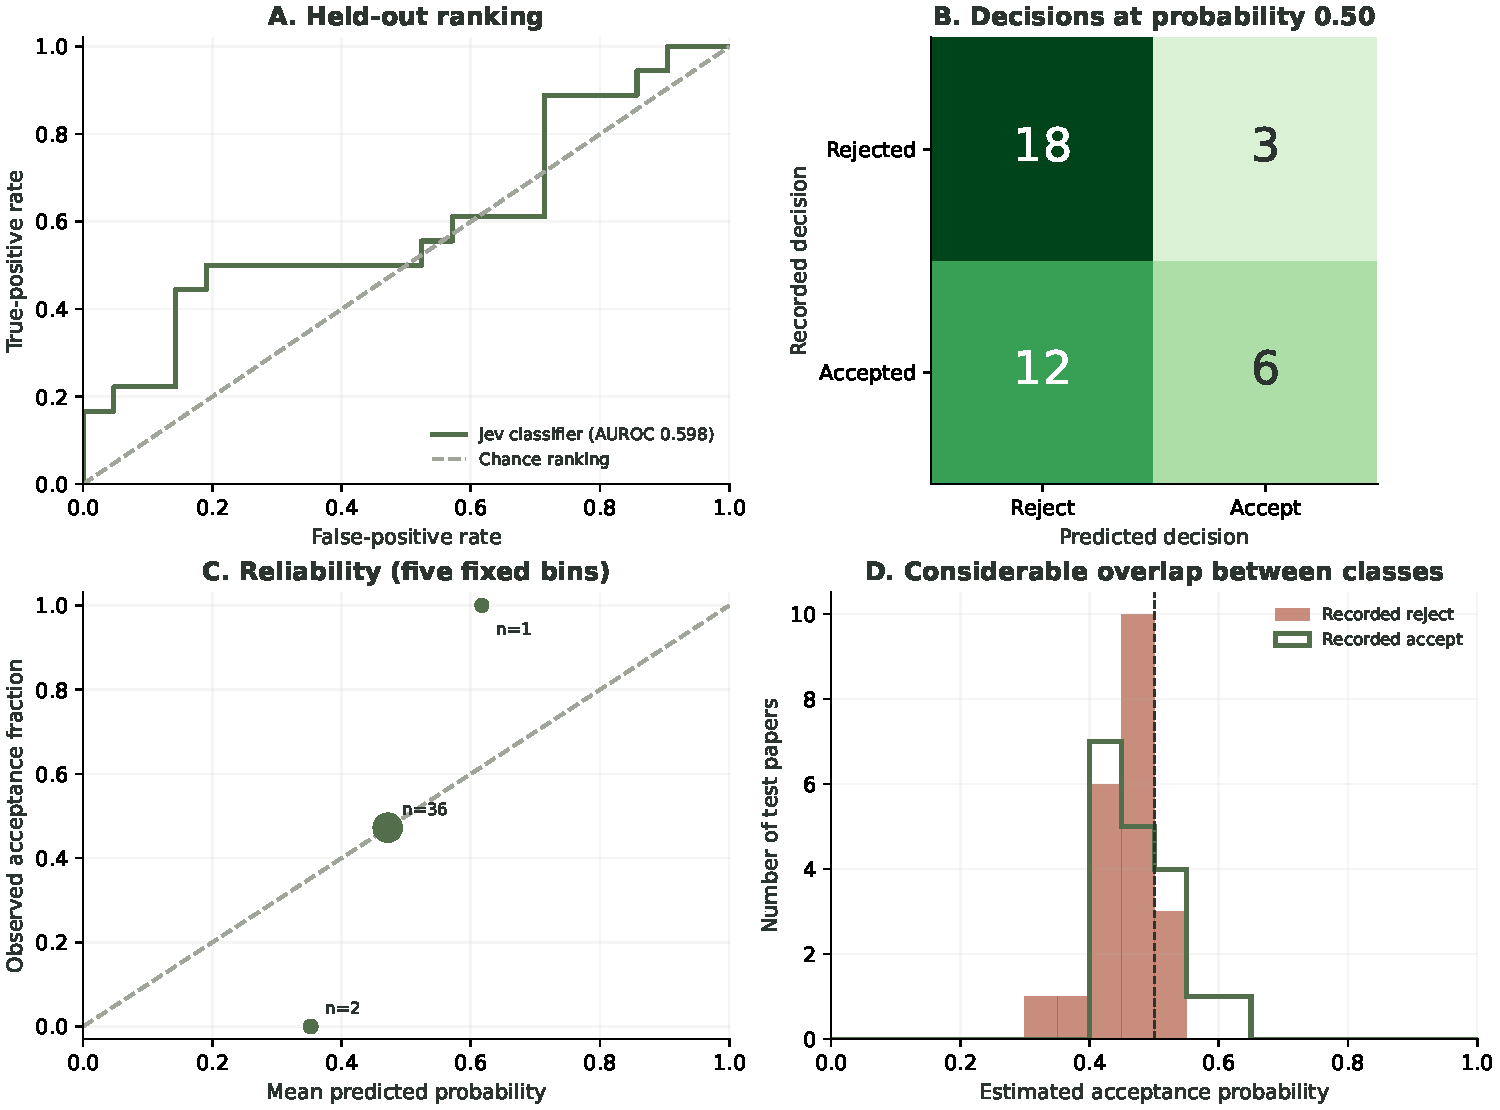
\includegraphics[width=\linewidth]{iclr2026-evaluation.pdf}
\caption{Untouched test predictions. The reliability plot uses five equal-width probability bins and omits empty bins; small counts make its points unstable. Class overlap and missed accepted papers limit practical usefulness. All panels derive from the exported study records.}
\end{figure}

\section{Live interface and engineering validation}
The authorized pilot downloaded at most 200 PDFs and evaluated 191 unique papers: 3,782 sections and 4,370 Jev passage requests, using 18,037,875 input tokens and 327,750 output tokens. Cached per-paper outputs allow scoring to resume and the classifier to be refitted without repeating paid inference. The initial scoring run completed in approximately six minutes in this environment. No monetary cost is inferred from token counts.

The interface visibly separates manuscript rubric scores, Jev output concentration, and the trained probability estimate. It shows test accuracy and the baseline, six recommendation bands, a binary prediction, validation intervals, limitations, and an expandable browser of accepted and rejected source papers. It identifies uploaded papers matching training, calibration, or test fingerprints; a training-paper result is explicitly marked as non-independent. Matching metadata is displayed after prediction and is not an input to the classifier.

The estimate becomes unavailable if the selected venue, research profile, Jev version, rubric, or selected guidance differs from training, or if required sections are incomplete. Other venues continue to receive section reviews and rubric scores. Reuploading or changing venues clears the old prediction. Exports include the estimate, model identity, validation results, and limits. The current engineering suite covers 114 backend tests and 30 desktop/mobile browser scenarios, including all six bands, incomplete streams, repeated uploads, label isolation, sklearn/runtime numerical agreement, source resolution, exports, and automated accessibility checks. Fixtures are separate from live research results.

Two additional live uploads of the same already-scored held-out PDF each refreshed the source timestamp and produced a distinct review identifier. They completed all twelve sections in 2.16 and 1.83 seconds, with first feedback at 1.28 and 0.95 seconds. Acceptance estimates were 42.3\% and 42.5\%, both ``Weak reject.'' These repeated integration observations are not new independent test examples and do not change the frozen evaluation. Screenshots use the recorded live response; automated browser fixtures remain separate.

\section{Interpretation and next study}
This pilot delivers an operational Jev-based reviewer and a trained, inspectable acceptance predictor. Its present predictive value is weak. Final decisions are noisy organizational outcomes, not scientific truth; the archive is selected rather than a representative draw from all submissions. Camera-ready content can leak post-decision information, and unknown pretraining overlap can inflate retrospective associations. No new-paper acceptance guarantee or independent section-quality validation follows from these measurements.

The next defensible study should obtain public submission-time versions with verified timestamps, retain actual final decisions separately, group manuscript revisions across splits, and hold out a later venue edition. It should increase sample size, report precision/recall and probability calibration, compare against simple writing/length baselines, inspect extraction failure rates by class, and assess memorization and prompt manipulation. Human section-level judgments would be required to validate the section reviewer itself. The current frozen test should remain an evaluation artifact, not become a tuning set.

\section{Reproducibility}
Run \texttt{npm run dev} and open \url{http://127.0.0.1:5173}. The server requires a configured Jev API key; secrets remain outside the browser. The training entry point is:
\begin{verbatim}
uv run python scripts/train_openreview.py --stage prepare --limit 200
uv run python scripts/train_openreview.py --stage score
uv run python scripts/train_openreview.py --stage fit
uv run --with matplotlib python scripts/plot_openreview.py
\end{verbatim}
The first stage uses pinned metadata and PDFs; the second incurs Jev inference; the third operates on cached numeric outputs. The JSON model is \texttt{artifacts/iclr2026-model.json}; paper-level decisions and held-out predictions are in \texttt{reports/iclr2026-study.json}; all numeric features are in \texttt{reports/iclr2026-features.json}. Selected guidance and raw responses are retained locally under \texttt{data/openreview/iclr2026}. Live reupload observations are recorded separately in \texttt{reports/iclr2026-live-validation.json}. Repeating external calls can change scores; matching version and guidance fingerprints are enforced rather than silently mixing runs.

Earlier general-review and NeurIPS integration experiments remain documented in \texttt{reports/findings.tex}; their rubric versions and results are separate from this supervised pilot.

\begin{thebibliography}{9}
\bibitem{jev} TypeSafe AI. \emph{Introduction and HTTP API reference}. Accessed 19 September 2026. \url{https://docs.typesafe.ai/introduction}; \url{https://docs.typesafe.ai/api}.
\bibitem{features} TypeSafe AI. \emph{Autoresearch feature discovery}. \url{https://docs.typesafe.ai/cookbooks/autoresearch_feature_discovery}.
\bibitem{iclr} ICLR. \emph{ICLR 2026 Reviewer Guide}. \url{https://iclr.cc/Conferences/2026/ReviewerGuide}. Venue: \url{https://openreview.net/group?id=ICLR.cc/2026/Conference}.
\bibitem{mirror} Weathon. \emph{ICLR 2026 public OpenReview mirror}. Pinned revision specified in the data-provenance section and machine-readable manifest. \url{https://huggingface.co/datasets/weathon/iclr_2026}.
\bibitem{copilot} Paper Copilot. \emph{Paper lists: ICLR 2026}. Pinned revision specified in the data-provenance section. \url{https://github.com/papercopilot/paperlists}.
\bibitem{calibration} Scikit-learn. \emph{Probability calibration}. \url{https://scikit-learn.org/stable/modules/calibration.html}.
\end{thebibliography}
\end{document}
